\documentclass{../../cursuspresentatie}

\def\importslide#1#2{%
	\import{../../slides/#1}{#2}
}

\title{GSNS \LaTeX{} course}
\author{\TeX niCie}
\date{8 September 2022}

% Als je het bestand dumpt naar een format, worden packages hierna niet meegedumpt maar elke keer
% fris ingeladen
\csname endofdump\endcsname

\usepackage{minted} %kan later in de .cls file hierboven
\usepackage{pdfpages}
\begin{document}

\section{Introduction}

\begin{frame}
	\titlepage
	\centering

	Please log in (or create an account) on \url{overleaf.com}
\end{frame}

\begin{frame}
	\frametitle{\lang,Schedule,Agenda,}
	
	\begin{itemize}
		\item \lang,Introduction to LaTeX and Overleaf,Introductie tot LaTeX en Overleaf,
		\item \lang,Text formatting,Tekstopmaak,
		\item  $ \langle $\lang,Exercises!,Oefeningen!,$ \rangle $
		\item \lang,Structure of a document,Documentstructuur,
		\item $ \langle $\lang,Exercises!,Oefeningen!,$ \rangle $
		\item \lang,Formulas,Formules,
		\item $ \mathbf\langle $\lang,Exercises!,Oefeningen!,$ \rangle $
		\item  \lang,Images,Afbeeldingen,
		\item $ \mathbf\langle $\lang,Exercises!,Oefeningen!,$ \rangle $
		\item \lang,Closing remarks,Afsluitende opmerkingen,
	\end{itemize}
\end{frame}

\begin{frame}
	\frametitle{Overleaf}
	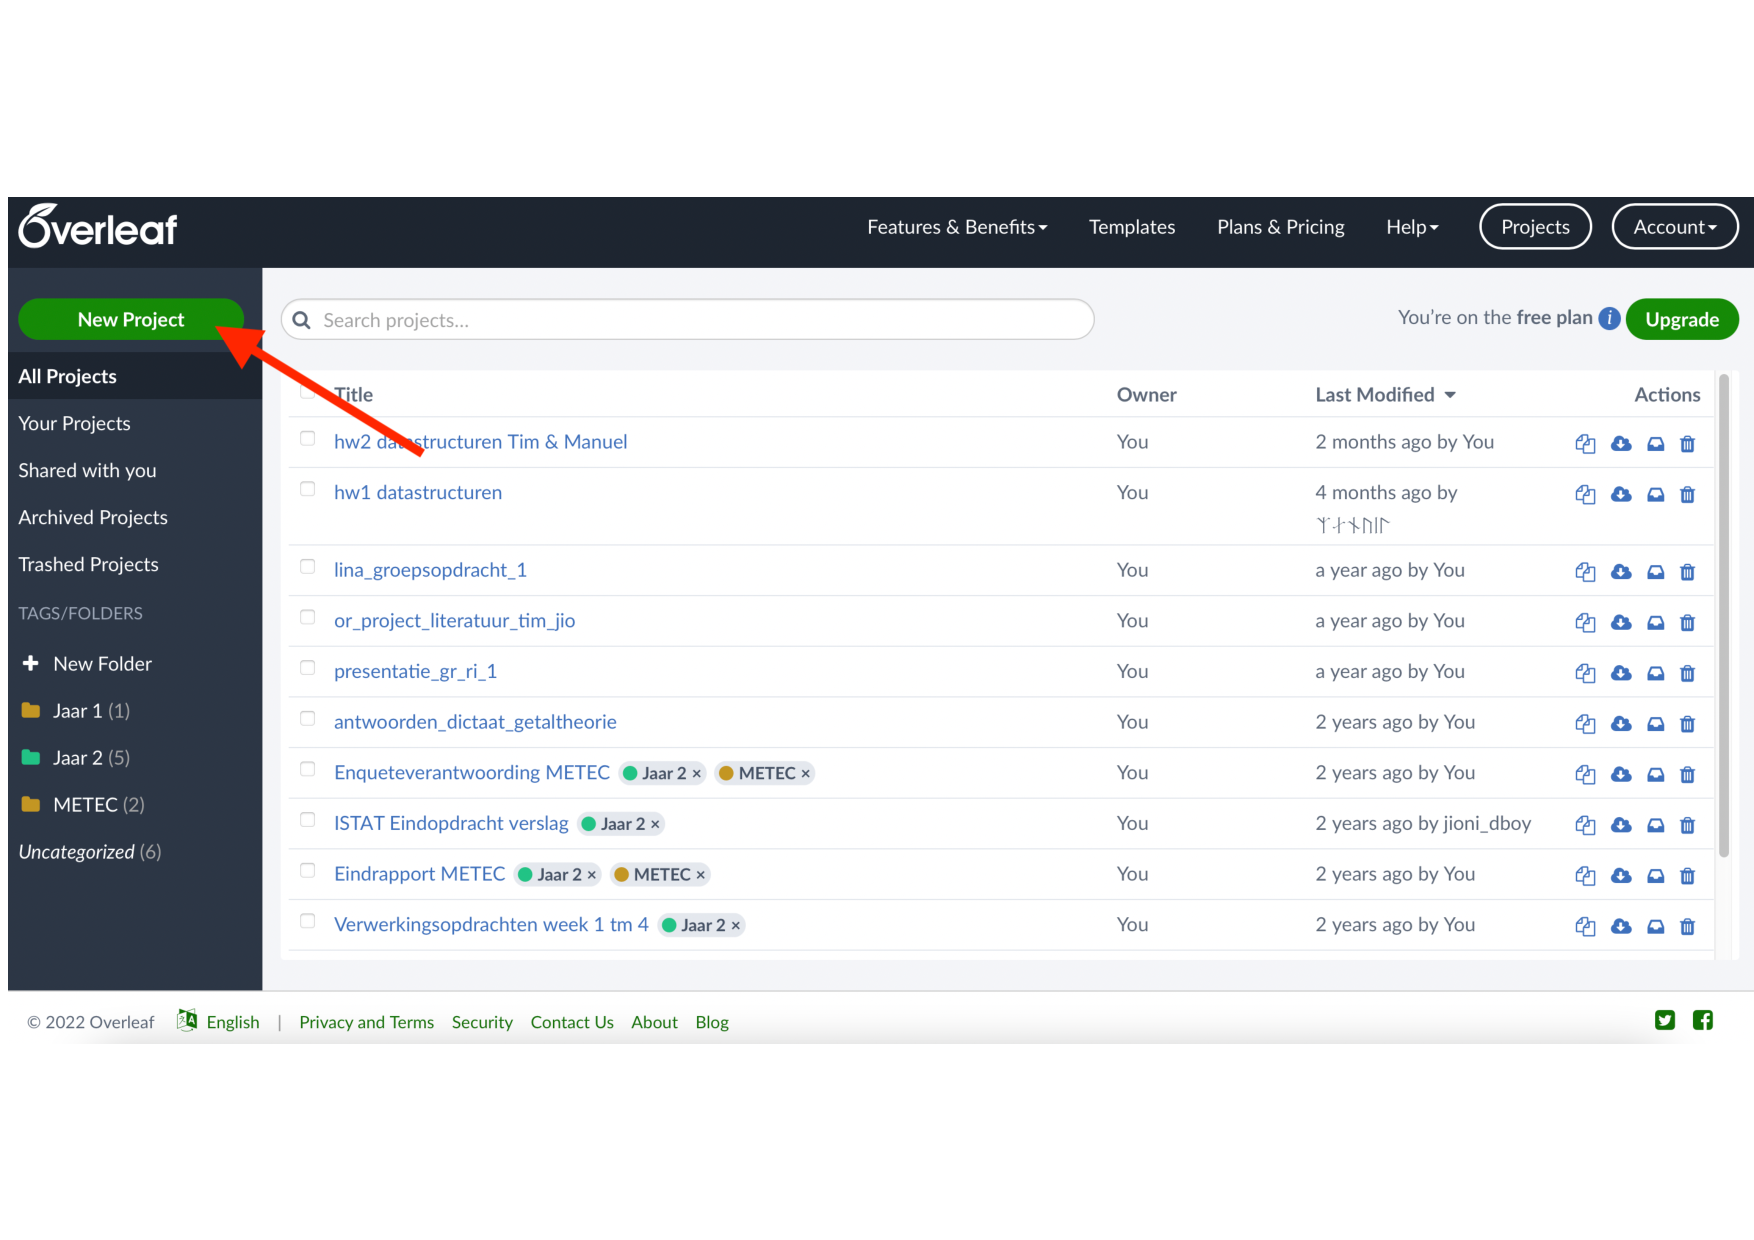
\includegraphics[width=1\textwidth]{images/overleaf_startscherm}
\end{frame}

\begin{frame}
	\frametitle{Overleaf}
	\begin{columns}
		\begin{column}{0.4\textwidth}
		  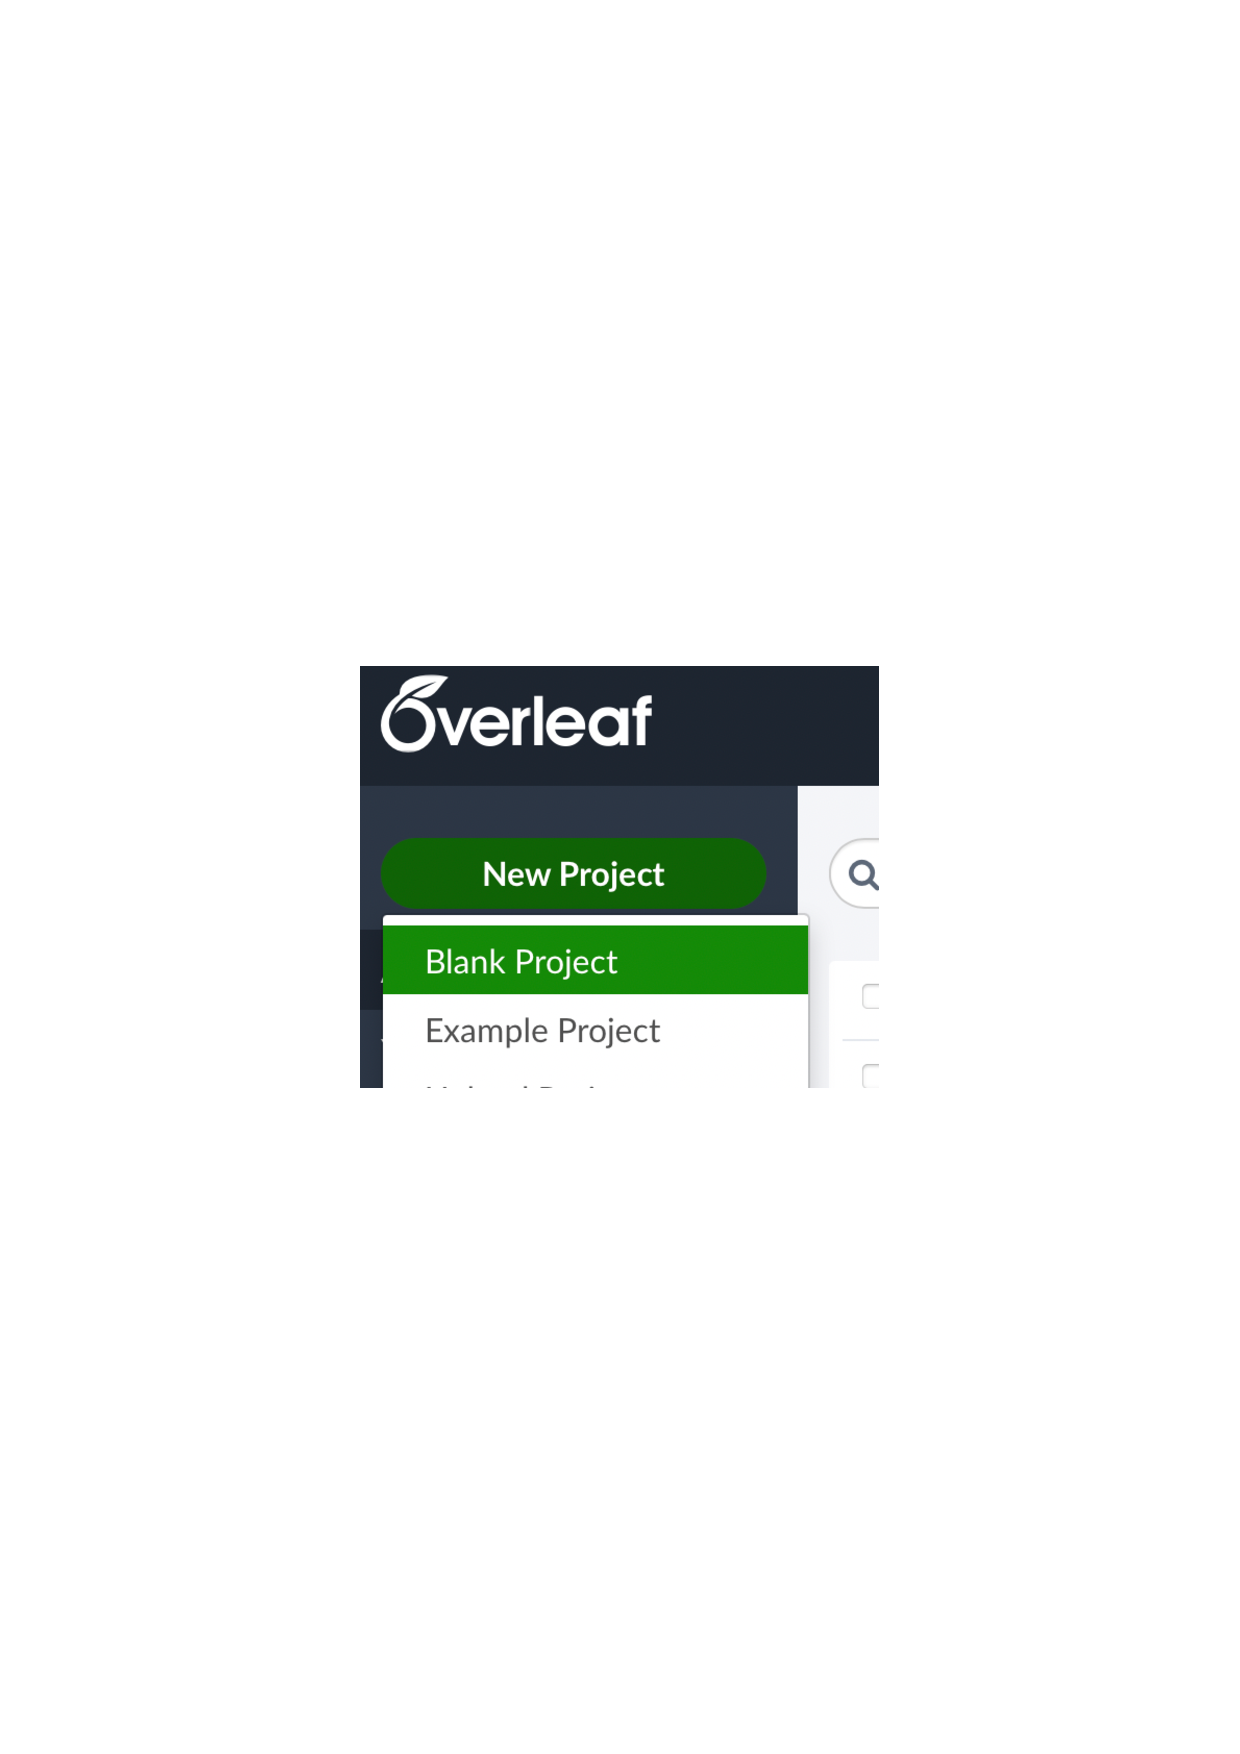
\includegraphics[width=0.8\textwidth]{images/new_project.pdf}\hfill
		\end{column}
		\begin{column}{0.4\textwidth}
		  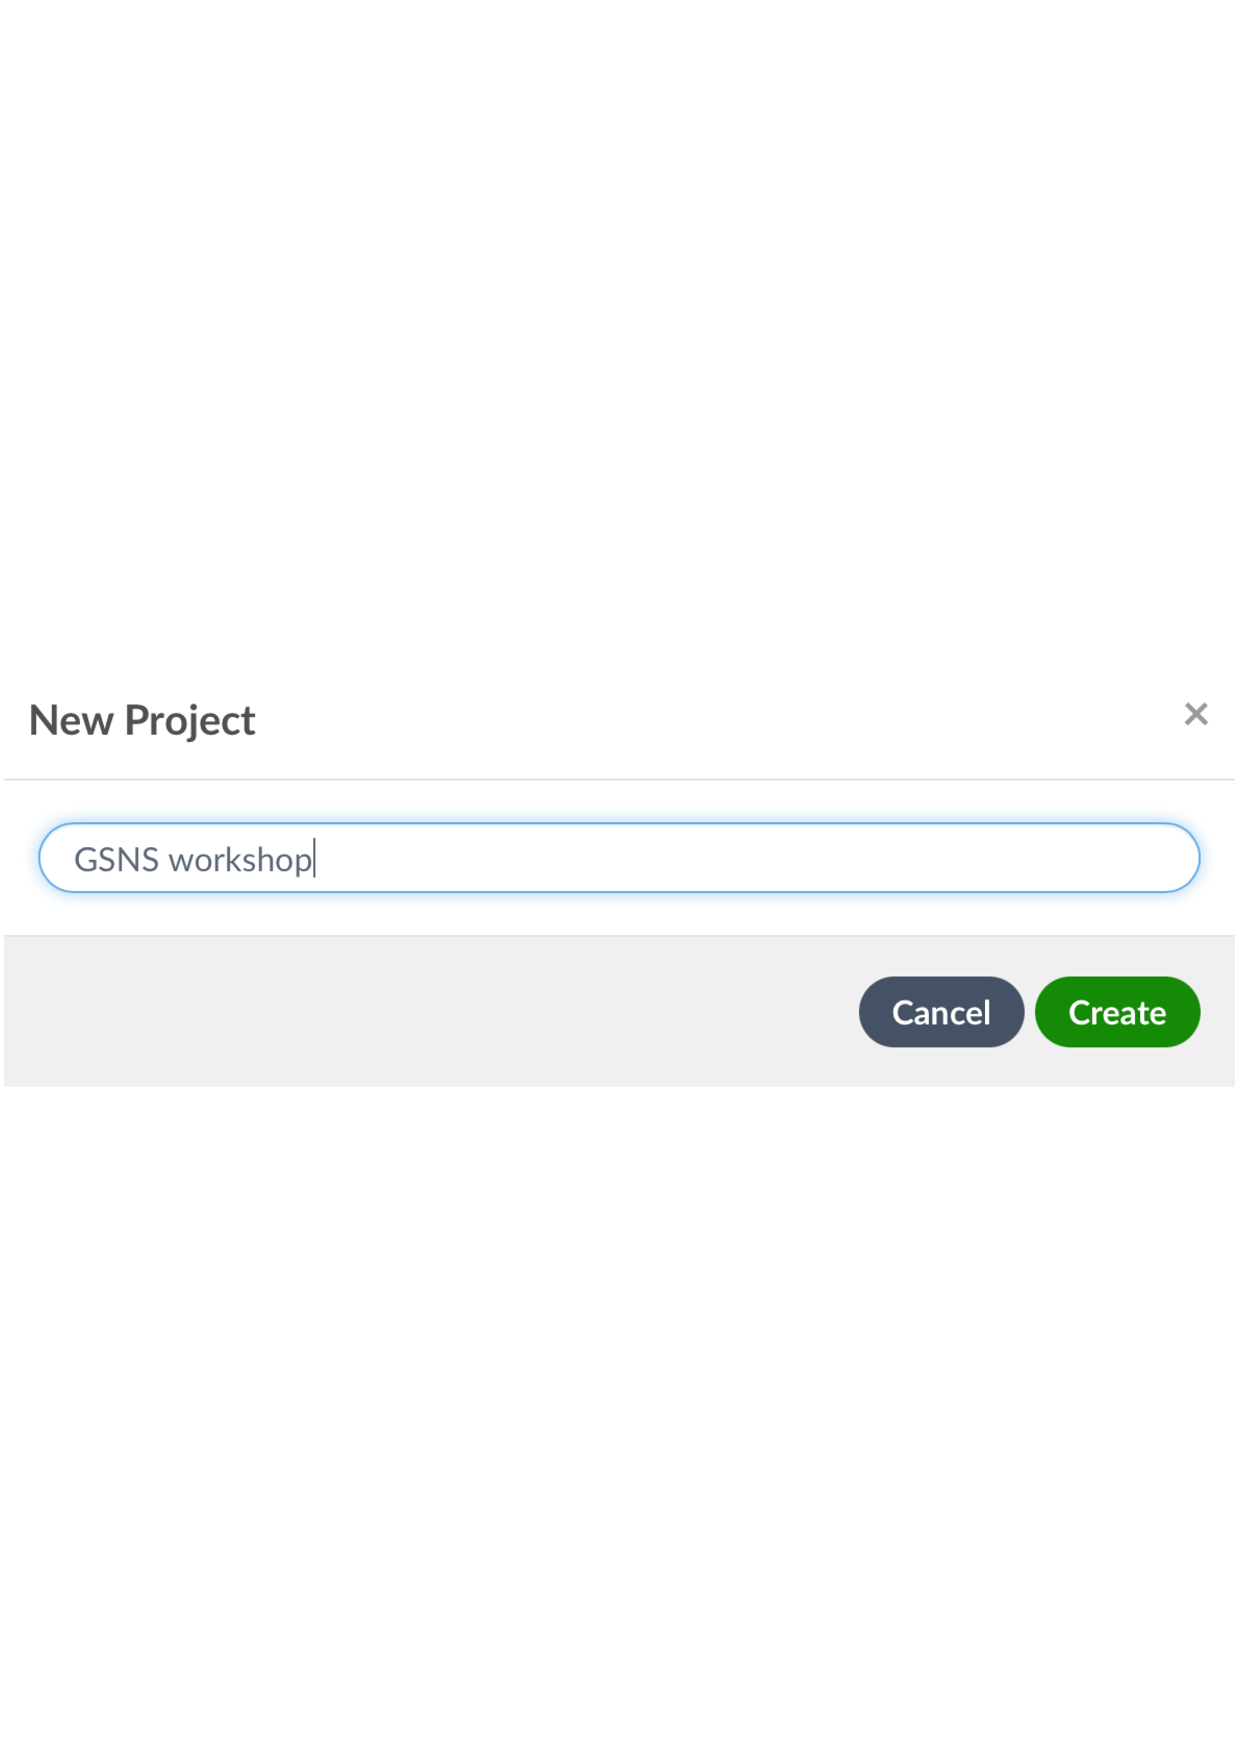
\includegraphics[width=1\textwidth]{images/project_name.pdf}
		\end{column}
	\end{columns}
\end{frame}

%TODO We switchen naar Overleaf voor Live LaTeX

\importslide{beginners}{beginners-simpledoc-1.tex}
\importslide{beginners}{beginners-simpledoc-2.tex}
\importslide{beginners}{beginners-simpledoc-3.tex}




% \subfile{1_Inleiding.tex}

% \subfile{2_Tekstopmaak.tex}

% \subfile{3_Documentstructuur.tex}

% \subfile{4_Afbeeldingen.tex}

% \subfile{5_Formules.tex}

% \subfile{6_Bibliografie.tex}

%\subfile{7_GoedOmTeWeten.tex}
	
\end{document}
